\Chapter{Mesh Adaptation Solver}

\modinfo{Module name}{included in solver}
\modinfo{Module subroutines}{\Idx{MeshSolver}}
\begin{versiona}
\modinfo{Module authors}{Juha Ruokolainen}
\modinfo{Document authors}{Juha Ruokolainen}
\modinfo{Document edited}{April 5th 2002}

\section{Introduction}

Moving boundaries are often encourtered in different types of computations,
i.e. Fluid-Structure-Interaction (FSI) problems.
Moving boundaries pose the problem of mesh adaptation to the boundaries.
With this solver, instead of generating the
whole mesh afresh when a boundary is moved, the current mesh nodes are moved
so that the mesh hopefully remains 'good'. This type of solution only applies
to cases where the changes in geometry are relatively small. It is, however, 
often cheaper in terms of CPU time to use this module in contranst to regenerate
the whole mesh.

For time dependent simulations the mesh deformation velocity is also computed.
The name of this variable is {\tt Mesh Velocity}.

\section{Theory}

The equation for elastic deformation of the mesh, given displacement of the boundaries,
may be written as
\begin{equation}
-\nabla\cdot {\bf \tau} = 0,
\end{equation}
where, $\Vec{d}$ is the mesh displacement field and $\tau$ the stress tensor.

The stress tensor given in terms of Lame parameters is:
\begin{equation}
\tau = 2 \mu \varepsilon + \lambda\nabla\cdot\Vec{d} I
\end{equation}
where $\mu$ and $\lambda$ are the first and second Lame parameters respectively,
and $I$ is the unit tensor.
The linearized strains are given as:
\begin{equation}
\varepsilon = \frac{1}{2}(\nabla{\Vec{d}} + (\nabla{\Vec{d}})^T).
\end{equation}
Lame parameters in terms of Youngs modulus and
Poisson ratio read
\begin{equation}
 \mu = \frac{Y \kappa}{( 1 - \kappa ) ( 1-2\kappa )},\ \ \  
 \lambda = \frac{Y}{2(1+\kappa)}
\end{equation}
Quantities $Y$ and $\kappa$ are the Youngs modulus and Poisson ratio respectively.
Note that in this context the values of the material parameters are fictional, and may
be chosen to help convergence or quality of the resulting mesh.


\subsection{Boundary Conditions}

For each boundary a Dirichlet boundary condition
\begin{equation}
d_i = d_i^b
\end{equation}
may be given. Usually this the displacement is given a priori or computed
by, for example, the elasticity solvers.

\section{Keywords} 
\end{versiona}

\sifbegin

\sifitem{Solver}{solver id} 
Note that all the keywords related to linear solver (starting
with {\tt Linear System})
may be used in this solver as well.  They are defined elsewhere. 

\sifbegin
\sifitem{Equation}{String [Mesh Update]} 
The name of the equation.
\sifend

\sifitem{Equation}{eq id}
The equation section is used to define a set of equations for a body or set of bodies:
\sifbegin
\sifitem{Mesh Update}{Logical} if set to {\tt True}, solve the mesh adaptation equations.
\sifend

\sifitem{Material}{mat id}
The material section is used to give the material parameter values. The
following material parameters may be set in Navier equations.
\sifbegin
\sifitem{Poisson Ratio}{Real} 
For isotropic materials Poisson ratio must be given with this keyword.
\sifitem{Youngs Modulus}{Real} The elastic modulus must be given with this
keyword.
\sifend


\sifitem{Boundary Condition}{bc id}
The boundary condition section holds the parameter values for various
boundary condition types. Dirichlet boundary conditions may be
set for all the primary field variables. The one related to Navier equations
are
\sifbegin
\sifitem{Mesh Update i}{Real} 
Dirichlet boundary condition
for each displacement component {\tt i}$=1,2,3$.
The boundary displacement may be computed some other solver. The computed
displacment field then may be used in the setting in the following way:
\sifitemnt{Mesh Update i}{Equals Displacement i}
with \texttt{i=1,2,3}.
Including such lines in the boundary condition setting will give
the mesh update on the boundary directly from the displacement solver.
\sifend
\sifend


\begin{versiona}
\section{Examples}

\subsection{A Simple FSI computation using MeshSolver}

In this simple computation Navier-Stokes equations are solved in the
domain shown in the two pictures below. On the left there is an inflow
boundary, and on the right an outflow boundary. In the block inside
the flow domain (the mesh is not shown for the block), the elasticity
equations are solved. The block is fixed at the bottom, and is otherwise
deformed by the fluid pressure and flow fields. The whole system is
iterated as follows:
\begin{itemize}
\item Solve fluid flow,
\item Solve deformation of the block,
\item Solve the fluid domain mesh with MeshSolver  according to the displacements
   of the block,
\end{itemize}
until convergence is obtained.

\begin{figure}[tbhp]
  \centerline{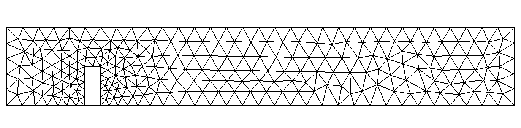
\includegraphics[width=0.7\textwidth]{orig.png}}
  \centerline{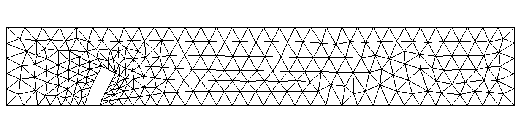
\includegraphics[width=0.7\textwidth]{deform.png}}
  \caption{The original computational mesh (up), and the mesh of the converged solution (down) of a FSI
    computation.}
\end{figure}

%\bibliography{elmerbib}
%\bibliographystyle{plain}

\end{versiona}
